\documentclass{article}
\usepackage[utf8]{inputenc}

\title{Mesterséges neuronhálók EA 1}
\author{Lörincz András elöadása alapján}
\date{2015 09 14}

\usepackage{natbib}
\usepackage{graphicx}

\begin{document}

\maketitle

\section{A tudományág kialakulása}
A mesterséges neuronhálók elméletének elsö lökését Donald O. Hebb, kanadai pszichológus adta 1949-ben, "The Organization of Behavior" cimü könyvében, melyben felvázolta a tanulásnak a neurális elméletét. Ebben azt posztulálta, hogy az agy biokémiai és elektromos folyamatokal változtatja saját struktúráját. Amikot két neuron egy idöben bocsát ki jelet, összeköttetésük erösödik, amikor koordinálatlanul tüzelnek, akkor gyengül (Hebb's postulate). \newline

\begin{figure}[h!]
\centering
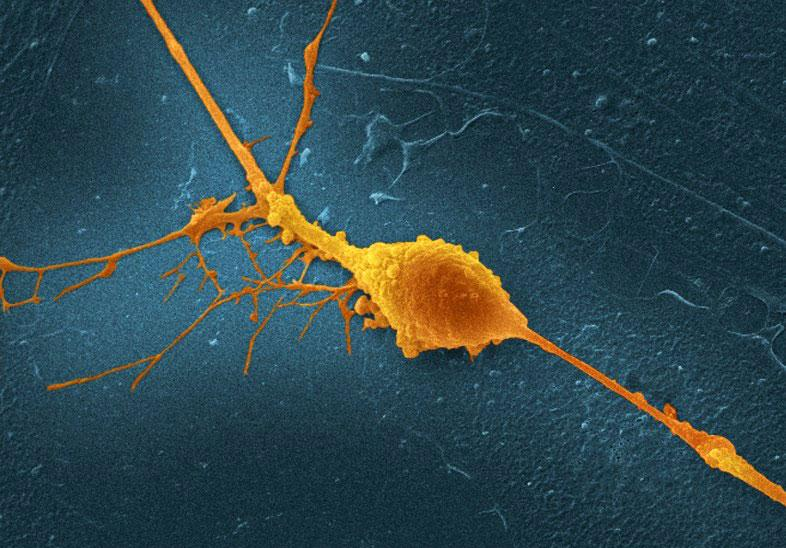
\includegraphics[width=\textwidth,height=\textheight,keepaspectratio]{realneuron.jpg}
\caption{A neuron elektronmikroszkópos képe}
\label{fig:realneuron}
\end{figure}

\begin{figure}[h!]
\centering
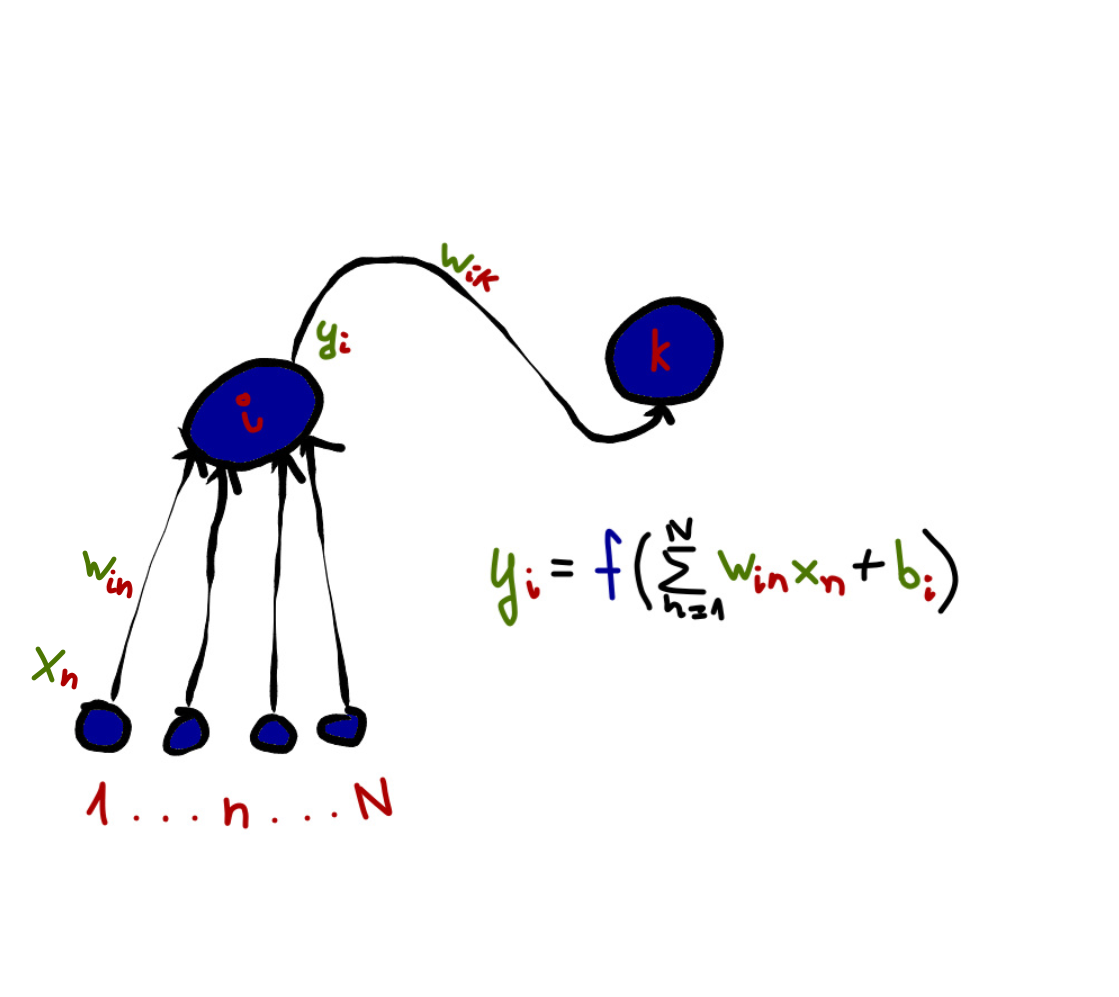
\includegraphics[width=\textwidth,height=\textheight,keepaspectratio]{abstractneuron.png}
\caption{A neuron absztrakciója}
\label{fig:abstractneuron}
\end{figure}

\section{Biológiai, pszichológiai alapok}
Az agy energiafelhasználása az egész test energiafelhasználásának közel 20\%-át teszi ki. Ennek felét a fehérállomány, felét a szürkeállomány adja. Agyunk nagyságrendileg $10^{11}$ neuront tartalmaz, de közel sem használja ki az összes kapcsolódási lehetöséget, csak $10^{14}$ kapcsolattal rendelkezik, ami neurononként 1000 kapcsolatot jelent. \newline

\begin{figure}[h!]
\centering
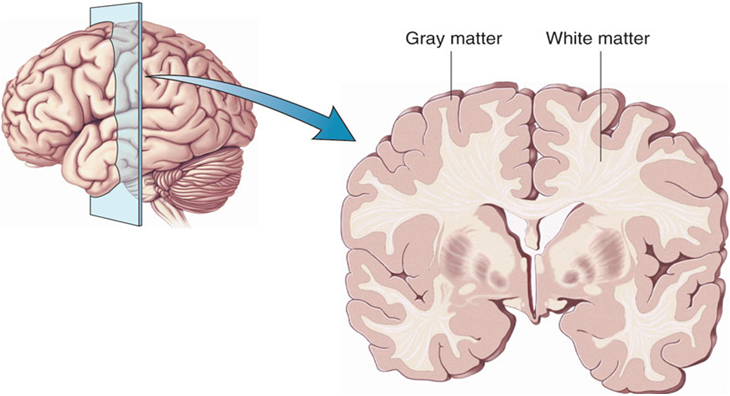
\includegraphics[width=\textwidth,height=\textheight,keepaspectratio]{brain.png}
\caption{Az agy fehér és szürkeállományának megoszlása}
\label{fig:brain}
\end{figure}

A neuronoknak a külvilágból érkezö jeleket (input) meg kell kapniuk az érzékszerveiktöl, és továbbitaniuk az izmoknak (output). Ez a folyamat akár fél másodpercet is igénybevehet, és nagy a variancia köztük. Ezt a problémát az agy poliszinkronizációval oldja meg, azaz a jeleket prediktálja és szinkronizálja, ami után az eltérés már néhány ms-ra lecsökken. \newline

További problémát jelent, hogy az agynak interpretálnia kell a jelet valahogyan, értelmes végeredményt kell kapnia. Ez paradoxonokhoz vezet. Pl. vegyünk két különbözö képet (majom és banán), és vetitsük a jobb és bal retinára öket egyszerre. Ekkor azt fogjuk tapasztalni, hogy a tesztalanyunk ahelyett, hogy egy összemosódott képet látna a kettö keverékéböl, kb. 700ms késleltetéssel látja elöször az egyik, aztán a másik képet, folyamatosan váltakozva. \newline

A kisérlet lényegét bár nem olyan látványosan, de könnyen lehet szemléltetni az alábbi képpel (fig. 4). Mit látunk? Nyulat, vagy kacsát? \newline

\begin{figure}[h!]
\centering
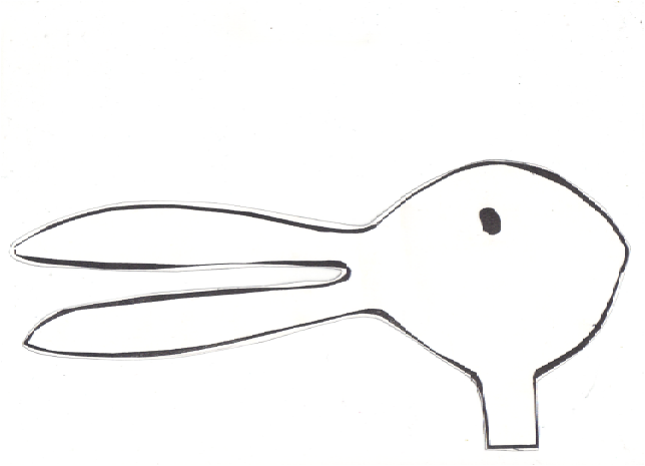
\includegraphics[width=\textwidth,height=\textheight,keepaspectratio]{duckrabbit.png}
\caption{An oldie but a goodie - It always comes back to the duck.}
\label{fig:duckrabbit}
\end{figure}

Ahhoz, hogy megértsük az inputokat milyen módon dolgozza fel az agy, egy hasznos segéd az úgynevezett "homunculus paradoxon", mely egy filozófiai eszköz elméletekben rejlö ellentmondások felismerésére. A pradoxon igy szól: az agyunknak muszáj a környezetét és saját állapotát valahogyan reprezentálnia. A probléma az, hogy ezt a  reprezentációt aztán értelmezni is kell. Viszont magának az interpretációnak is valahogyan reprezentálva kell lennie. Ezt is interpretálni kell és igy tovább. Ennek feloldása, hogy az értelmezést nem a reprezentáción végezzük, hanem maga a reprezentáció értelmezi azt amit reprezentál. Ha a reprezentációból le lehet vezetni az inputot, akkor értelmes, ha nem, akkor nem. \newline

\begin{figure}[h!]
\centering
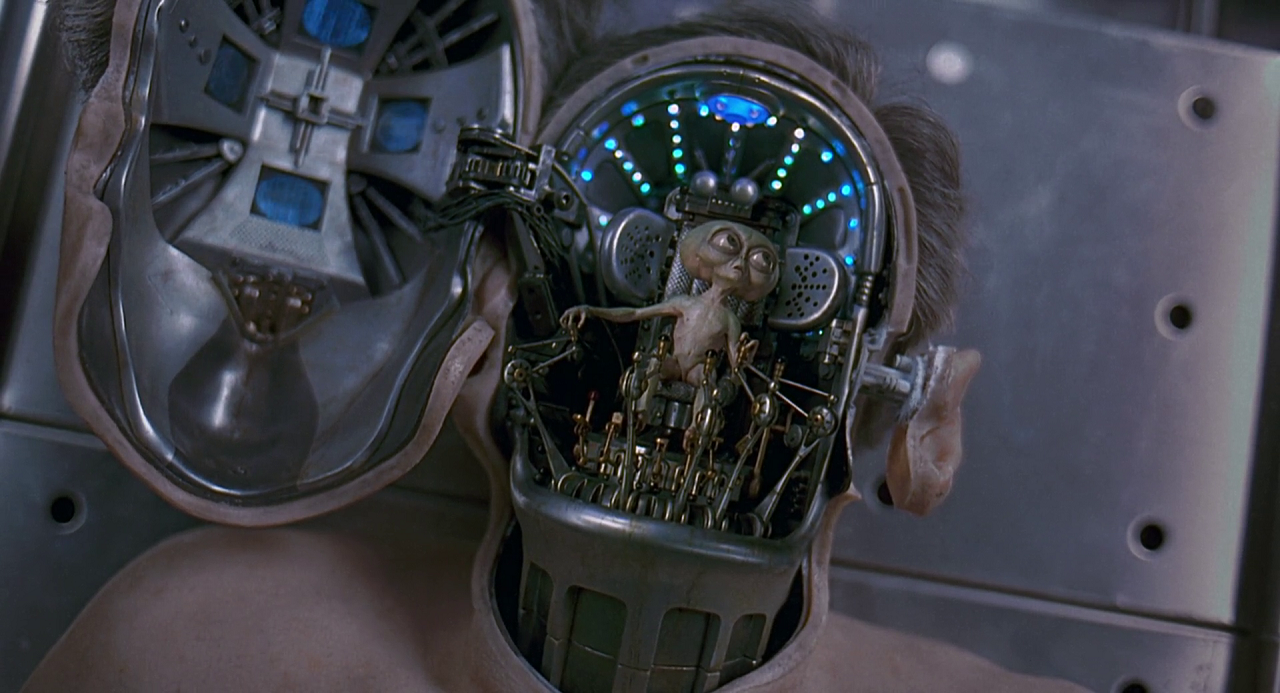
\includegraphics[width=\textwidth,height=\textheight,keepaspectratio]{homunculus.png}
\caption{Homunculus}
\label{fig:homunculus}
\end{figure}

\section{Fogalmak}
$y_i = f(\sum_{n=1}^N w_{in}*x_n + b_i)$ \newline

Neuron: $y_i$ az i. neuron képlete. Az inputokat megszorozza az i. sullyal, ezeket mind osszeadja, eltolja a $b_i$-vel, végül az egész leképzödik a kivánt range-be az aktivációs függvény (f) által. \newline

Súlyvektor: az összes $w_i$ súlyoknak a vektora. A kapcsolat erösségét jelzik. \newline

Küszöb: képletünkben $b_i$ az i. küszöb. Ez segit eltolni függvényünket, hogy a neuron ne legyen túl érzékeny. \newline

A küszöböt fel lehet irni a sulyvektor komponenseként is. Ekkor képletünk leegyszerüsödik: $y_i = f(\sum_{n=0}^N w_{in}*x_n)$, ahol $x_0 = 1$, igy megkapjuk az eredeti képletet $w_{i0} = b_i$ esetén. \newline

Nemlinearitás: A valódi neuronok nemlineáris dinamikus rendszerként müködnek. Ennek a modellnek a reprezentálásához olyan függvényeket használunk, mint a sigmoid, vagy a tanh függvény. \newline

Sigmoid: $\frac{1}{(1+e^{-t})}$ \newline

Tanh: $\frac{e^x-e^{-x}}{e^x+e^{-x}}$ \newline

Osztályozás: A neurális háló outputja valami diszkrét osztályok egyikét adja vissza. Például angol ábécé karaktereinek felismerése: 26 elemü osztály valamelyikébe sorolja az inputot. \newline

Short Term Memory (STM): aktuális aktivitás-mintázat \newline

Long Term Memory (LTM): az összes információ a bementtöl a kimenetig \newline

\end{document}
